\documentclass[tikz]{standalone}

\usepackage[latin1]{inputenc}
\usepackage{tikz}

% GNUPL
\begin{document}

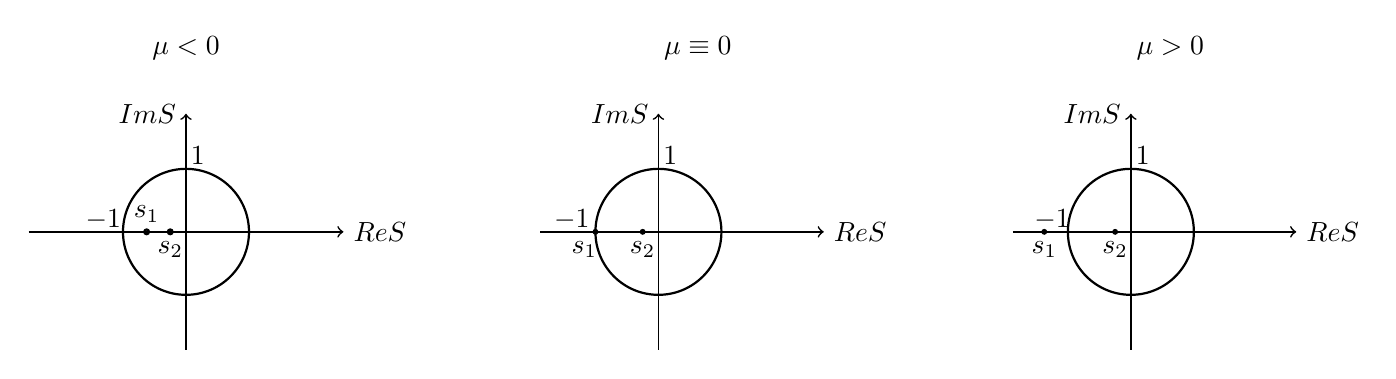
\begin{tikzpicture}
    % \draw[very thin,color=gray] (20,10) grid (0,0);
    % \foreach \x in {0,1,2,3,45,6,7,8,9,10,11,12,13,14,15,16,17,18,19,20}
    % \draw (\x cm,1pt) -- (\x cm,-1pt) node[anchor=north] {$\x$};
    % \foreach \y in {0,1,2,3,4,5,6,7,8,9,10}
    % \draw (1pt,\y cm) -- (-1pt,\y cm) node[anchor=east] {$\y$};
    %\mu<0
    \coordinate [label=-90:$\mu<0$] (8) at (2.5,8.6);
    \draw[semithick] [->] (0.5,6) -- (4.5,6) node[right] {$Re{S}$};
    \draw[semithick] [->] (2.5,4.5) -- (2.5,7.5) node[left] {$Im{S}$};
    \draw[thick] (2.5,6) circle [radius=0.8];
    \coordinate [label=-90:$1$] (8) at (2.65,7.2);
    \coordinate [label=-90:$-1$] (8) at (1.45,6.4);
    \draw[thick] (2.3,6) circle [radius=0.03];
    \draw[thick] (2,6) circle [radius=0.03];
    \coordinate [label=-90:$s_2$] (8) at (2.3,6);
    \coordinate [label=90:$s_1$] (8) at (2,6);
	%\mu=0
    \coordinate [label=-90:$\mu \equiv0$] (8) at (9,8.6);
    \draw[semithick] [->] (7,6) -- (10.6,6) node[right] {$Re{S}$};
    \draw[semithick] [->] (8.5,4.5) -- (8.5,7.5) node[left] {$Im{S}$};
    \draw [fill] (8.3,6) circle [radius=0.03];
    \draw [fill] (7.7,6) circle [radius=0.03];
    \draw[thick] (8.5,6) circle [radius=0.8];
    \coordinate [label=-90:$1$] (8) at (8.65,7.2);
    \coordinate [label=-90:$-1$] (8) at (7.4,6.4);
    \coordinate [label=-90:$s_2$] (8) at (8.3,6);
    \coordinate [label=-90:$s_1$] (8) at (7.56,6);
    %\mu>0
    \coordinate [label=-90:$\mu>0$] (8) at (15,8.6);
    \draw[semithick] [->] (13,6) -- (16.6,6) node[right] {$Re{S}$};
    \draw[semithick] [->] (14.5,4.5) -- (14.5,7.5) node[left] {$Im{S}$};
    \draw [fill] (14.3,6) circle [radius=0.03];
    \draw [fill] (13.4,6) circle [radius=0.03];
    \draw[thick] (14.5,6) circle [radius=0.8];
    \coordinate [label=-90:$1$] (8) at (14.65,7.2);
    \coordinate [label=-90:$-1$] (8) at (13.5,6.4);
    \coordinate [label=-90:$s_2$] (8) at (14.3,6);
    \coordinate [label=-90:$s_1$] (8) at (13.4,6);
\end{tikzpicture}


\end{document}